\section{Theoretische Grundlage}
\label{sec:Theorie}
Unter dem Zeemaneffekt wird die Aufspaltung von Spektrallinien im Magnetfeld bezeichnet, sowie die Polarisation des Lichtes verstanden. Dabei wird zwischen dem normalen und dem anomalen Zeemaneffekt differenziert. Im folgenden wird die theoretische Grundlage des Versuches skizziert.

\subsection{Magnetisches Moment eines Elektrons}
Elektronen besitzen sowohl einen Bahndrehimpuls $l$ sowie einen Eigendrehimpuls $s$. In der weiteren Betrachtung werden nur die Drehimpulse der äußeren Schalen der Atome betrachtet, da die der abgeschlossenen Schalen in Summe verschwinden. Ausgehend von der Eigenwertgleichung der Zustände des Atoms werden die Beträge der Quantenzahlen zu
\begin{eqnarray}
  |\vec{l}| = \sqrt{l(l+1)} \hbar  \\
  |\vec{s}| = \sqrt{s(s+1)} \hbar
  \label{eqn:betQua}
\end{eqnarray}
berechnet. Dabei laufen der Bahndrehimpuls $l$ von 0, 1, \ldots $\,$ n-1 und der Spin $s$ ist $\frac{1}{2}$. Für die Berechnung der magnetischen Momenten wird das Borsche Magneton $\mu_\text{B}$ eingeführt welches eine Art infinitesimales magnetisches Moment ist. Es entspricht dem magnetischen Moment welche ein Elektron mit $l$=1 erzeugt. Das in Maßeinheiten des Magnetons berechnete magnetische Momente des Bahndrehimpulses beträgt
\begin{equation}
  \vec{\mu_\text{L}} = -\mu_\text{B} \sqrt{l(l+1)} \vec{l_\text{e}} \ .
  \label{eqn:magL}
\end{equation}
Bei der Einführung des magnetischen Moment des Spins $\mu_\text{s}$
\begin{equation}
  \mu_\text{s} = - \mu_\text{B} g_\text{S} \sqrt{s(s+1)} \vec{s_\text{e}}
  \label{eqn:magS}
\end{equation}
tritt der Landé-Faktor $g_\text{S}$ auf, auf welchen im folgenden noch weiter eingegangen wird.

\subsection{Wechselwirkungen der Drehimpulse untereinander}
Bei den Wechselwirkungen der einzelnen Drehimpulse untereinander wird zwischen zwei verschiedenen Fällen unterschieden, die fließend ineinander übergehen.  Bei dem ersten Fall wird davon ausgegangen, dass die Kernladungszahl niedrig ist. Die Wechselwirkungen zwischen den einzelnen $\vec{l_\text{i}}$ ist so groß, dass ein Gesamtdrehimpuls $\vec{L}$ eingeführt werden kann.
\begin{equation}
  \vec{L} = \sum \vec{l_\text{i}}
  \label{eqn:L}
\end{equation}
In Analogie zu den einzelnen Drehimpulsen wird das magnetische Moment
\begin{equation}
  |\mu_\text{L}| = \mu_\text{B} \sqrt{L(L+1)}
  \label{magL}
\end{equation}
des Gesmatbahndrehimpuls eingeführt. Analog zum Bahndrehimpuls wird auch eine Gesamtspinquantenzahl $S$ als auch ein magnetisches Moment $\mu_\text{S}$ eingeführt . Für nicht zu großen Magnetfelder lässt sich der Gesamtdrehimpuls $\vec{J}$ aus der Summe von $L$ und $S$ einführen welcher auch als LS-Kopplung bezeichnet wird.
Der zweite Fall der Kopplung von Spin und Bahndrehimpuls wird als j-j-Kopplung bezeichnet. Dabei wird angenommen, dass bei schweren Atomen die Wechselwirkung des Spins und des Bahndrehimpulses untereinander so groß wird, dass diese nicht mehr vernachlässigt werden kann. Somit müssen die einzelnen Gesamtdrehimpulse
\begin{equation}
  \vec{j_\text{i}} = \vec{l_\text{i}} + \vec{s_\text{i}}
  \label{eqn:j}
\end{equation}
berücksichtigt werden, sodass der Gesamtdrehimpuls $\vec{J}$ die Summe der einzelnen $\vec{j_\text{i}}$ ist.

\subsection{Aufspaltung der Energieniveaus}
Das magnetisches Moment des Gesamtdrehimpulses ist die Summe der magnetischen Momente des Spins $\mu_\text{s}$ und des Bahndrehimpulses $\mu_\text{l}$.
\begin{equation}
  \mu = \mu_\text{s} + \mu_\text{l}
\end{equation}
Da der Landé-Faktor bei Elektronen welche ein Spin 1/2 haben, in etwa den Wert 2 besitzt, zeigen $\mu$ und $J$ im Regelfall nicht in die gleiche Richtung. Dies hat zur folge, dass das magnetischen Moments in einen Anteil welches sich Parallel zum Gesamtdrehimpuls befindet $\mu \parallel J$ und einem welches sich antiprallel $\mu \nparallel J$ zum Gesamtdrehimpuls befindet zerlegt werden kann. Für die Messzeiten präzidiert der  $\mu \nparallel J$ Anteil, so schnell um den Gesamtdrehimpuls $J$ herum, dass der $\mu$ welches sich antiparallel zu $J$ befindet im zeitlichen Mittel wegfällt. Der parallele Anteil $\mu \parallel J$ wird im weiteren Verlauf $\mu_\text{J}$ genannt. Für den Betrag von $\mu_\text{J}$ ergibt sich
\begin{equation}
  |\vec{\mu_\text{J}}| = \mu_\text{B} g_\text{J} \sqrt{J(J+1)} \ ,
  \label{eqn:muJ}
\end{equation}
wobei $g_\text{J}$ der Landé-Faktor ist. Dieser ist definiert als
\begin{equation}
  g_\text{J} = \frac{3J(J+1) + S(S+1) -L(L+1)}{2J(J+1)}
  \label{eqn:Lan}
\end{equation}
Im folgenden wird angenommen, dass ein äußeres B-Feld in Z-Richtung anliegt. Die Richtungsquantelung besagt, dass bei angelegtem Magnetfeld nur solche Winkel auftreten, bei dennen die Projektion von $\mu_\text{J}$ auf das B-Feld ein ganzzahliges vielfache von $g_\text{J} \mu_\text{B}$ auftritt.
\begin{equation}
  \vec{\mu} = -m g_\text{J} \mu_\text{B}
  \label{eqn:mu}
\end{equation}
Dabei kann die Orientierungsquantenzahl $m$ die Werte $(-J, \cdots, J)$ annehmen. Somit Spalten sich die Energieniveaus im Magnetfeld in $2J+1$ Niveaus auf, deren Energiedifferenzen zum Magnetfeldfreien Niveau
\begin{equation}
	\Delta E_\text{mag} = m \vec{\mu_\text{B}} \vec{g_\text{J}}
  \label{eqn:delE}
\end{equation}
ist. Ein Beispiel für die Aufspaltung eines Niveaus mit $J=2$ ist in Abbildung \ref{fig:Eniv} zu sehen.
\begin{figure}
  \centering
  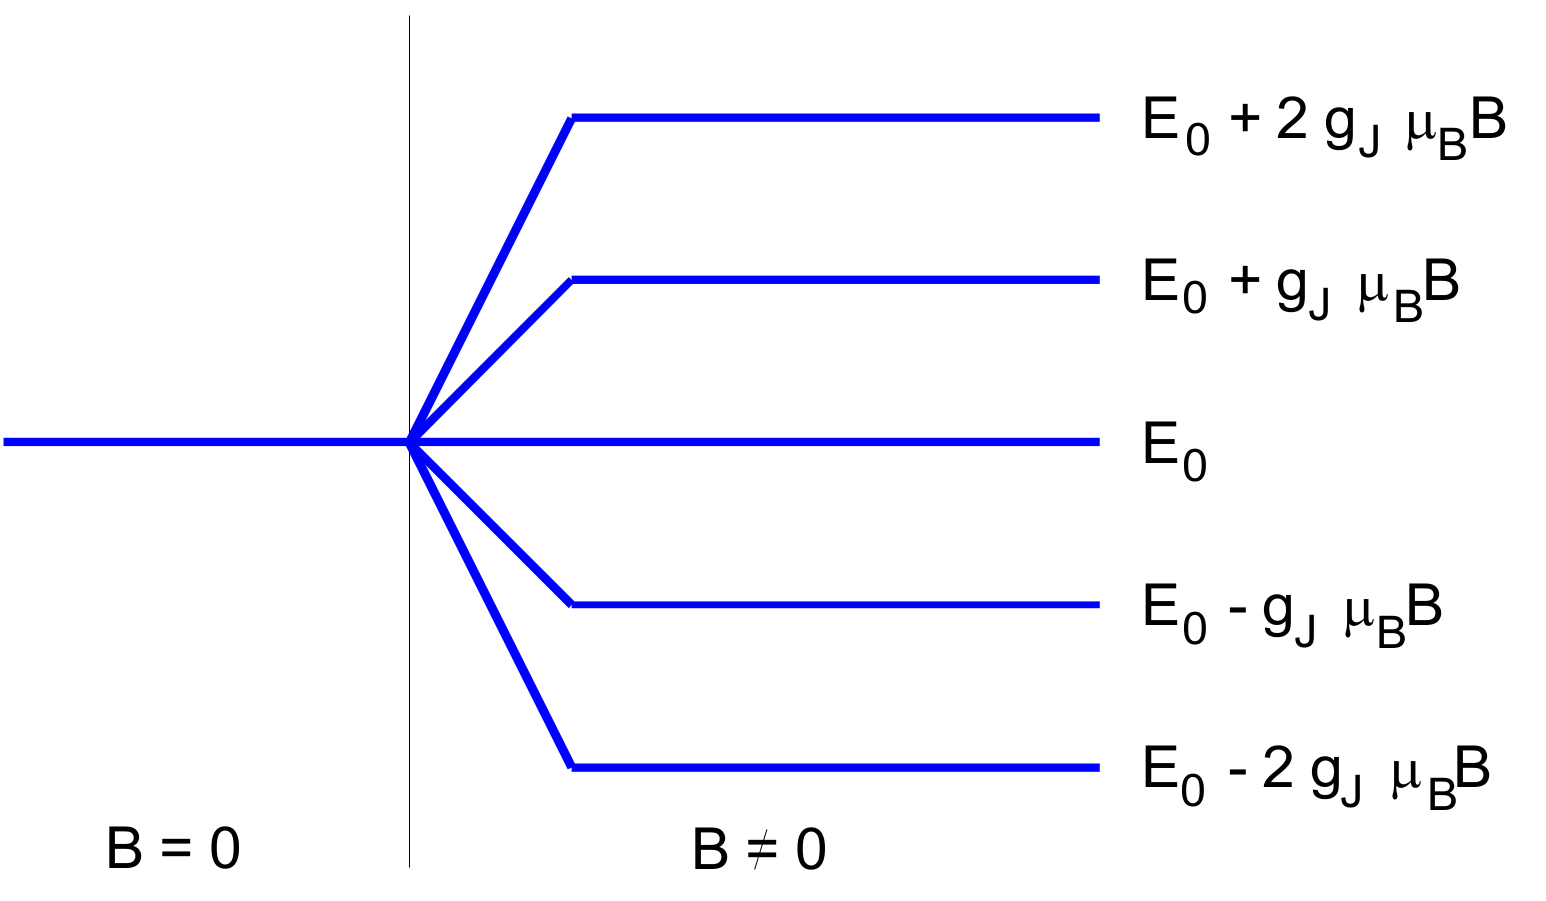
\includegraphics[height=6cm]{./Bilder/ENiveaus.png}
  \caption{Aufspaltung der Energieniveaus im Magnetfeld \cite{V27}}
   \label{fig:Eniv}
\end{figure}

\subsection{Auswahlregeln}
Mithilfe der Schrödingergleichung wird untersucht, welche Niveauübergänge möglich sind. Als Ansatz zur Lösung wird die Summe zweier ebener Wellen genommen, bei denen der Spin berücksichtigt wird. Aus der Dichtefunktion lässt sich die Schwingungsfrequenz $\nu_{\alpha\beta}$ der Elektronen von
\begin{equation}
  \nu_{\alpha\beta}= \frac{E_{\alpha} - E_{\beta}}{\hbar}
  \label{eqn:nu}
\end{equation}
herleiten. Zur Berechnung des Dipolmomentes muss das Integral
\begin{equation}
  -e_0\, \int x \, \Psi^* \Psi \, \text{dV}
  \label{}
\end{equation}
gelöst werden. Anhand der Lösung kann aus dem Poyntingvektor abgeleitet werden, dass alle Beiträge verschwinden, außer wenn $m$ die Zahlenwerte
\begin{equation}
  \Delta m = -1,0,1
\end{equation}
annimmt. Aus der Herleitung lässt sich schließen, dass bei Anlegung eines äußeren magnetischen Feldes für $m = 0$ das elektrische Feld des Lichtes $E_\text{Licht}$ entlang des B-Feldes ausgerichtet ist. Dieser Übergang wird $\pi$ Übergang genannt und ist nur in voller Intensität zu beobachten, wenn der Polfilter senkrecht zum angelegtem B-Feld steht und kann unterdrückt werden indem der Polarisationsfilter parallel zum Feld gestellt wird. \\
Ist die Orientierungsquantenzahl $m = \pm 1$, ist das E-Feld um die B-Feldachse zirkular polarisiert. Dieser Übergang wird $\sigma^{+/-}$ genannt, entsprechend des Vorzeichens von $m$ und ist aufgrund der zirkularpolarisation sowohl longitudinal als auch bei transversaler Betrachtung zu beobachten.
\begin{figure}[H]
  \centering
  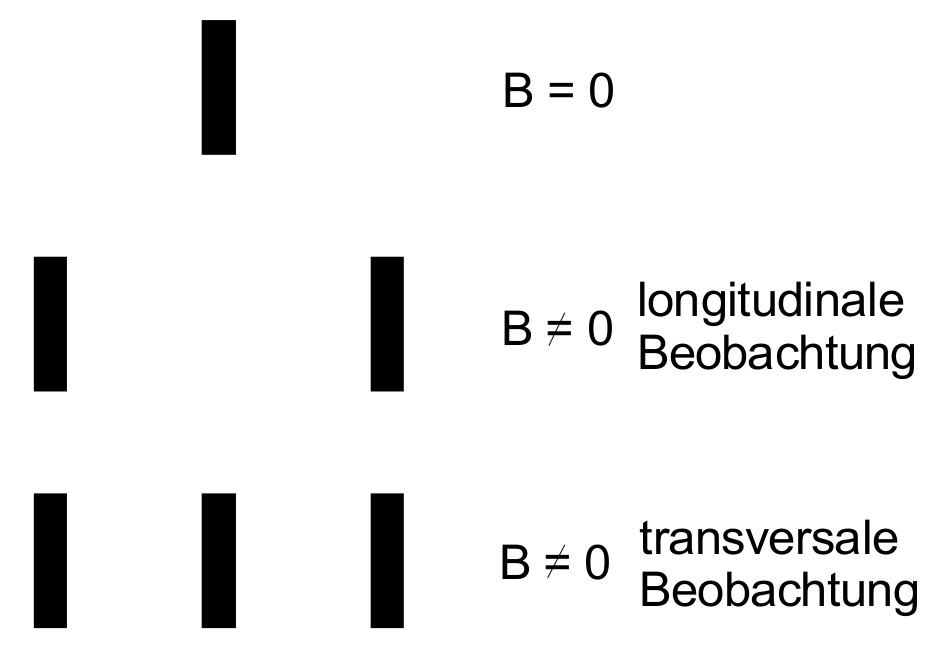
\includegraphics[width=0.8\textwidth]{./Bilder/Aufspaltung.png}
  \caption{Longitudinale und transversale Aufspaltung des Zeemaneffektes bei Anlegung eines äußeren B-Feldes \cite{V27}}
  \label{fig:aufZe}
\end{figure}
Der Abbildung \ref{fig:aufZe} ist zu entnehmen das zur identifizierung des $\pi$ Übergangs der Polfilter vertikal auszurichten ist. Zur Betrachtung des $\sigma$ Übergang muss dementsprechend der Polfilter horizontal ausgerichtet werden.
\subsection{Normaler Zeeman-Effekt}
Beim normalen Zeeman-Effekt verschwindet die Summe der einzelnen Spins ($S=0$), sodass der entsprechende Landé-Faktor, unabhängig von allen Quantenzahlen $L$ und $J$, $g_\text{J} = 1$ ist. Die Energiedifferenz der Übergänge kann mittels Formel \ref{eqn:delE} berechnet werden. Das Linenspektrum spaltet somit in $2 J + 1$ Linien auf.Eine Aufspaltung der Spektrallinie für J = 2 ist in Abbildung \ref{fig:Eniv} zu sehen.
Das Linienspektrum spaltet sich gemäß der Auswahlregeln in 3 Komponenten auf, sodass die $\sigma^{+/-}$ und $\pi$ Übergänge wie in Abbildung \ref{fig:adf} dargestellt detektierte werden können. 
\begin{figure}[H]
  \centering
  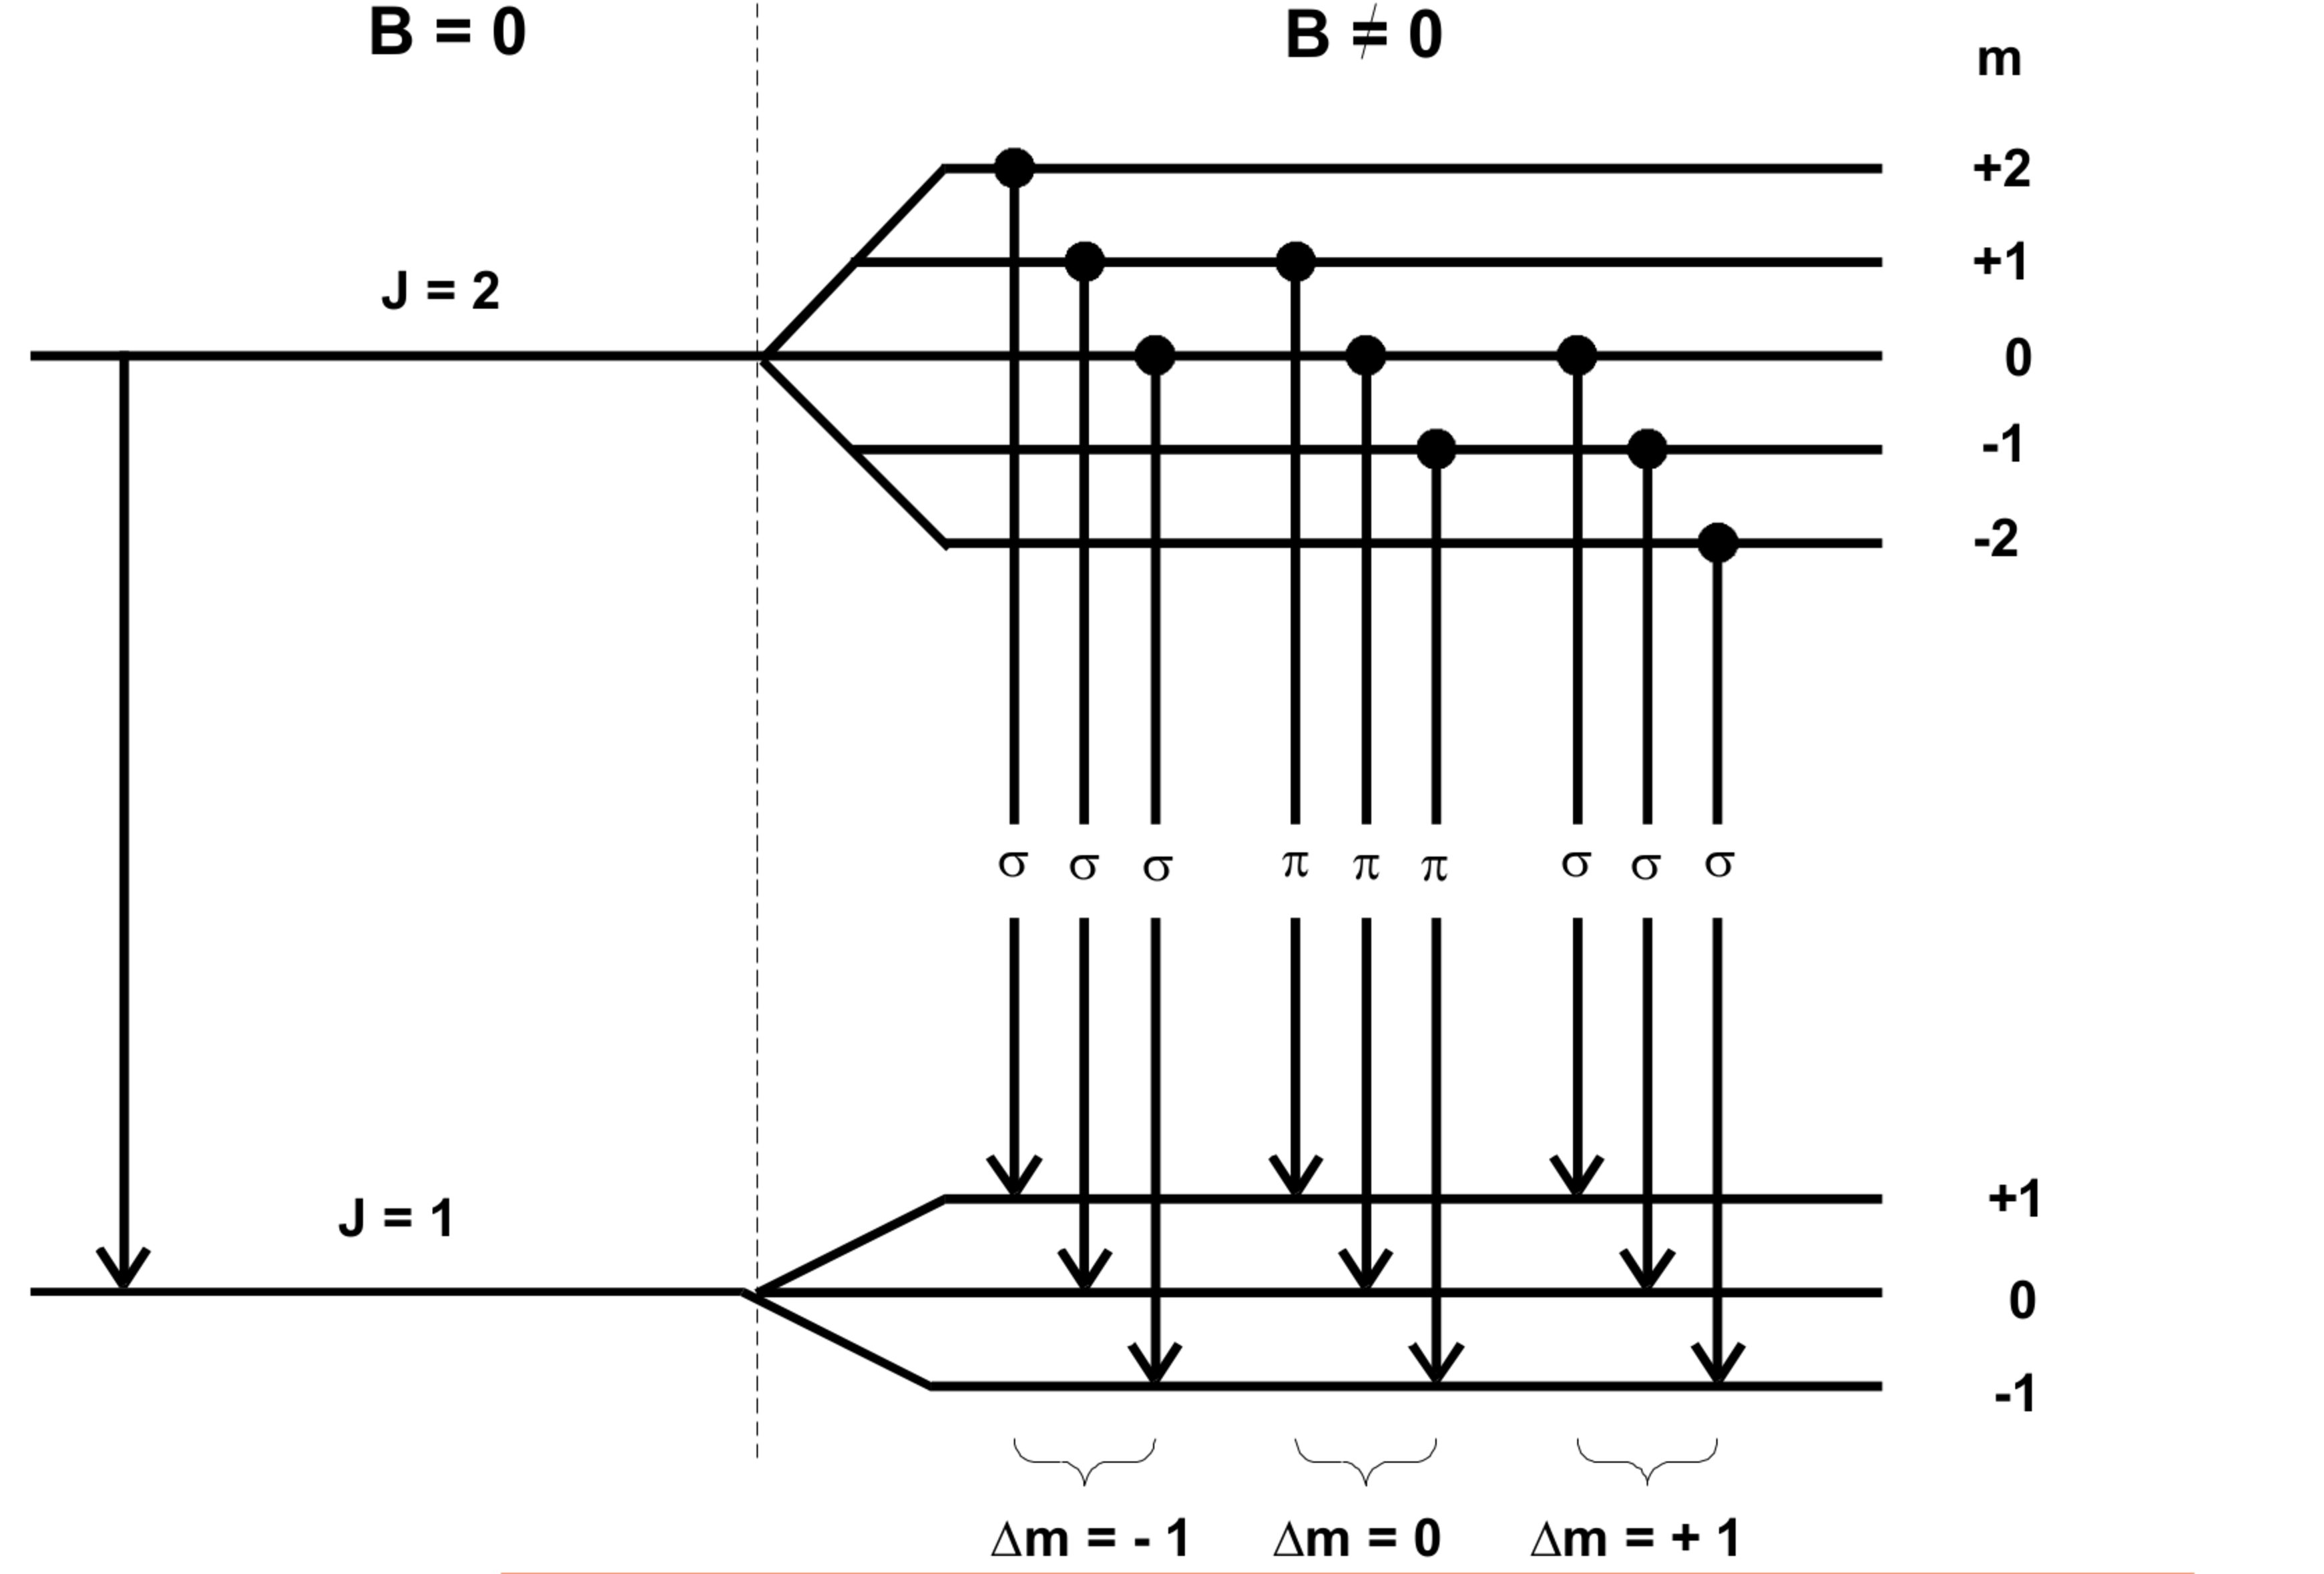
\includegraphics[width=0.6\textwidth]{./Bilder/asd.pdf}
  \caption{$\pi$ und $\sigma$ Übergänge beim normalen Zeeman-Effekt \cite{V27}}
  \label{fig:adf}
\end{figure}

\subsection{Anomaler Zeeman-Effekt}
Bei der Aufspaltung von Spektrallinien im Magnetfeld bei denen mindestens einer der beiden Zustände einen von Null verschiedenen Gesamtspin hat, wird vom Anomalen Zeeman-Effekt gesprochen. Den Anomaler Zeemaneffekt kennzeichnet das Landefaktoren auftreten, welche ungleich eins seien können. Die Energiedifferenz der einzelnen Niveaus lässt sich durch die Formel
\begin{equation}
  \Delta E = \mu_\text{B}\,B\,(m_1 g_1 + m_2 g_1)
  \label{eqn:dE}
\end{equation}
berechnen. Da die Landefaktoren von L, J und S abhängen gibt es in der Regel mehr Übergänge zwischen den Energieniveaus die detektiert werden können.



\subsection{Fehlerrechnung}
Sämtliche Fehlerrechnungen werden mit Hilfe von Python 3.4.3 durchgeführt. \\
Für die Berechnung der Mittelwerte wird die Funktion "mean" aus dem Paket Numpy genommen und für die Standardabweichung die Funktion "std". Für die Fehlerfortpflanzung wird das Paket "uncertainties \cite{uncertainties}" benutzt. \\
Als Fitfunktion wird "scipy.optimize.curve\_fit \cite{scipy}" verwendet.
